%---------------------------------------------------------------------------%
%-                                                                         -%
%-                          Beamer Template                                -%
%-                                                                         -%
%---------------------------------------------------------------------------%
%- Copyright (C) Huangrui Mo <huangrui.mo@gmail.com> 
%- This is free software: you can redistribute it and/or modify it
%- under the terms of the GNU General Public License as published by
%- the Free Software Foundation, either version 3 of the License, or
%- (at your option) any later version.
%---------------------------------------------------------------------------%
%->> Document class declaration
%---------------------------------------------------------------------------%
\documentclass[compress,table,aspectratio=169,xcolor={usenames,dvipsnames}]{beamer}%
%- Multiple options:
%- [<t|c|b>]% vertical alignment for content, vertically centered is default
%- [<slidestop|slidescentered>]% set frame titles position
%- [compress]% reduce the navigate bars
%- [<red|blue|brown|blackandwhite>]% set navigate bar color
%- [<10pt|11pt|12pt|14pt|17pt>]% set font size for normal text, 11pt is default
%- [table]% support tables
%- [aspectratio=169]% set aspect ratio to 16:9, and frame size to 160mm by 90mm
%- [aspectratio=1610]% set aspect ratio to 16:10, and frame size to 160mm by 100mm
%- [aspectratio=MN]% set aspect ratio to M:N, and frame size to 10*M mm by 10*N mm
%- [xcolor={usenames,dvipsnames}]% issue options to xcolor via a beamer-option
%- Manually adjust aspect ratio: design to 4x3, then expand to target, and live with empty space
%- \documentclass[aspectratio=169]{beamer}
%-     \beamertemplatenavigationsymbolsempty%
%-     \usepackage{pdfpages}%
%- \begin{document}
%-     \setbeamercolor{background canvas}{bg=}%
%-     \includepdf[pages=-]{my-original-presentation.pdf}%
%- \end{document}
%- The default font size may seem small, but the actual size of each frame size is
%- by default just 128mm by 96mm and the viewer application enlarges the frame and font.
%- By specifying a default font size smaller than 11pt one can put more onto each slide,
%- by specifying a larger font size one can fit on less.
%---------------------------------------------------------------------------%
%->> Document settings
%---------------------------------------------------------------------------%
\usepackage[biber,authoryear,tikz,table,xlink]{Style/artrabeamer}% document settings
%- usage: \usepackage[option1,option2,...,optionN]{artrabeamer}
%- Multiple optional arguments:
%- [CJK]% Chinese environment support
%- [bibtex|biber]% set bibliography processor and package
%- [<numbered|authoryear|alpha>]% set citation and reference style
%- <numbered>: textual: Jones [1]; parenthetical: [1]
%- <authoryear>: textual: Jones (1995); parenthetical: (Jones, 1995)
%- <alpha>: textual: not available; parenthetical: [Jon95]
%- [tikz]% provide complex diagrams via tikz package
%- [table]% provide complex tables via ctable package
%- [list]% provide enhanced list environments for algorithm and coding
%- [math]% enable some extra math packages
%- [showonlynote]% show note pages only
%- [showsecnote]% show note pages on second screen
%- [handout]% enable handout output
%- [xlink]% disable link colors
\usepackage{Style/artracom}% user defined commands
%---------------------------------------------------------------------------%
%->> Document inclusion
%---------------------------------------------------------------------------%
%\includeonly{Tex/Sec_Introduction}% selected files compilation
%\includeonlylecture{lecture label}% selected lectures compilation
%---------------------------------------------------------------------------%
%->> Theme settings
%---------------------------------------------------------------------------%

%%%%%%%%%%%%%%%% insert here our packages

% tree structure
\usepackage{forest}
%%%%%%%%%

\usepackage{subfigure}
\usepackage[font=tiny,labelfont=bf]{caption}
\usepackage[italian]{babel}


%-
%-> Recommended theme combinations
%-
%- set: [<usetheme>, <useoutertheme>, <useinnertheme>, <usecolortheme>]
%- light: [<CambridgeUS>, <miniframes>, <circle>, <dove|seahorse|beaver|seagull>]
%- light: [<Boadilla|Madrid>, <default>, <circle>, <dove|seahorse|beaver|seagull>]
%- dark: [<Boadilla|Madrid>, <default>, <circle>, <fly|albatross>]
%-
%-> Global themes
%-
\usetheme{CambridgeUS}%
%- Options:
%- [<Boadilla|CambridgeUS|default|...>]
%- It is the complete theme in the sense that they control just about every aspect
%- of a slide's appearance. Think of it as major theme.
%- Theme Matrix (https://www.hartwork.org/beamer-theme-matrix/) contains the
%- various theme and color combinations included with beamer.
%-
%-> Outer themes
%-
%\useoutertheme{}%
%- Options:
%- [<default|infolines|miniframes|smoothbars|sidebar|split|shadow|tree|smoothtree>]
%- An outer theme dictates (roughly) the overall layout of frames. It specifies where
%- any navigational elements should go (like a mini table of contents or navigational
%- mini frames) and what they should look like. Typically, an outer theme specifies
%- how the following elements are rendered:
%- - The headline and footline.
%- - The sidebars.
%- - The logo.
%- - The frame title.
%- The Beamer User Guide explains each theme with examples.
%-
%- *** Miniframes
\useoutertheme[%
    %footline=empty,% suppressed the footline (default).
    %footline=authorinstitute,% shows the author's name and the institute in the footline.
    %footline=authortitle,% shows the author's name and the title in the footline.
    %footline=institutetitle,% shows the institute and the title in the footline.
    %footline=authorinstitutetitle,% shows all three in the footline.
    subsection=false,% shows or suppresses line showing the subsection in the headline.
]{miniframes}%
%-
%- *** Sidebar
%\useoutertheme[%
%    %left,% sidebar links.
%    %right,% sidebar rechts.
%    %hideallsubsections,% suppresses all subsections.
%    %hideothersubsections,% suppresses all subsections except the current one.
%]{sidebar}%
%-
%-> Inner themes
%-
\useinnertheme{circles}%
%- Options:
%- [<default|circles|rectangles|rounded|inmargin>]
%- An inner theme installs templates that dictate how the following elements are typeset:
%- - Title and part pages.
%- - Itemize environments.
%- - Enumerate environments.
%- - Description environments.
%- - Block environments.
%- - Theorem and proof environments.
%- - Figures and tables.
%- - Footnotes.
%- - Bibliography entries.
%-
%-> Color themes
%-
\usecolortheme{dove}%
%- Options:
%- [<dove|seahorse|beaver|seagull|fly|albatross|...>]
%- Control the colors of title, frame title, itemization bullets,
%- and many other elements of a slide show.
%- More detailed configure:\setbeamercolor{beamer_element}{color} for
%- of Beamer elements, e.g.color setup
%\setbeamercolor{title}{fg=red!80!black,bg=red!20!white}
%\setbeamercolor{frametitle}{fg=blue,bg=yellow}
%---------------------------------------------------------------------------%
%->> Configuration
%---------------------------------------------------------------------------%
%-
%-> Set templates
%-
%- As a user of the beamer class you typically do not 'use' or 'invoke'
%- templates yourself, directly. For example, the frame title template
%- is automatically invoked by beamer somewhere deep inside the frame
%- typesetting process. The same is true of most other templates.
%- However, if, for whatever reason, you wish to invoke a template
%- yourself, you can use the following command.
%-\setbeamertemplate{some beamer element}{your definition for this template}
%-
%- *** Headline and footline
%\setbeamertemplate{headline}[infolines theme]
%\setbeamertemplate{footline}[page number]
%- Options: {},[default],[infolines theme],[miniframes theme],[frame number],
%-          [page number],[text line]{ text },...
%- Example for redefine the footline:
%-
%- First define some "beamer color" entries:
%\setbeamercolor{myentry1}{fg=black,bg=red!20}
%\setbeamercolor{myentry2}{fg=black,bg=red!30}
%\setbeamercolor{myentry3}{fg=black,bg=red!40}
%- Syntax for \begin{beamercolorbox}[options]{beamer color} ... \end{beamercolorbox}.
%- footline:
%\setbeamertemplate{footline}{
%  \leavevmode%
%  \hbox{%
%  \begin{beamercolorbox}[wd=.333333\paperwidth,ht=2.25ex,dp=1ex,center]{myentry1}%
%-    \usebeamerfont{author in head/foot}\insertshortauthor
%  \end{beamercolorbox}%
%  \begin{beamercolorbox}[wd=.333333\paperwidth,ht=2.25ex,dp=1ex,center]{myentry2}%
%-    \usebeamerfont{title in head/foot}\insertshorttitle
%  \end{beamercolorbox}%
%  \begin{beamercolorbox}[wd=.333333\paperwidth,ht=2.25ex,dp=1ex,right]{myentry3}%
%-    \usebeamerfont{date in head/foot}\insertshortdate{}\hspace*{2em}
%    \insertframenumber{} / \inserttotalframenumber\hspace*{2ex}
%  \end{beamercolorbox}}%
%  \vskip0pt%
%}
%- headline:
%\setbeamertemplate{headline}{
%  \leavevmode%
%  \hbox{%
%  \begin{beamercolorbox}[wd=.5\paperwidth,ht=2.65ex,dp=1.5ex,right]{myentry1}%
%    \usebeamerfont{section in head/foot}\insertsectionhead\hspace*{2ex}
%  \end{beamercolorbox}%
%  \begin{beamercolorbox}[wd=.5\paperwidth,ht=2.65ex,dp=1.5ex,left]{myentry3}%
%    \usebeamerfont{subsection in head/foot}\hspace*{2ex}\insertsubsectionhead
%  \end{beamercolorbox}}%
%  \vskip0pt%
%}
%- Change the footer/footline of a single frame in Beamer: use {} to confine effect domain.
%- The \leavevmode ensures that the vertical mode is ended and horizontal mode is entered. 
%- In vertical mode, TeX stacks horizontal boxes vertically, whereas in horizontal mode, 
%- they are taken as part of the text line. Use \leavevmode for all macros which could be 
%- used at the begin of the paragraph and add horizontal boxes by themselves.
%-
%- *** Outline setting
%\AtBeginPart% [<Lecture|Part|Section>]% insert content at the beginning of each element
%{%
%    \frame[plain]{\partpage}% [<partpage|sectionpage>][<\insertlecture|\insertpart|\insertsection>]
%    \begin{frame}[plain]%
%        \frametitle{Outline}%
%        {%
%            \tableofcontents[sectionstyle=show/shaded,subsectionstyle=show/show/shaded]%
%        }%
%    \end{frame}%
%}
%- - sectionstyle=<style for current section>/<style for other sections>
%- - subsectionstyle=<style for current subsection>/<style for other
%-   subsections in current section>/<style for subsections in other sections>
%- - Allowed <styles> are show, shaded, and hide.
%- Other options:
%- - currentsection, equal to: sectionstyle=show/shaded,subsectionstyle=show/show/shaded
%- - currentsubsection, equal to: subsectionstyle=show/shaded.
%- - firstsection=<section number> specifies which section should be numbered as section "1."
%-   This is useful if you have a first section (like an overview section) that should not
%-   receive a number.
%- - hideallsubsections, equal to: subsectionstyle=hide.
%- - pausesections, causes a \pause command to be issued before each section.
%-   This is useful if you wish to show the table of contents in an incremental way.
%-
%- *** Navigation symbols
\setbeamertemplate{navigation symbols}{}% suppresses all navigation symbols.
%\setbeamertemplate{navigation symbols}[only frame symbol]% only for navigating frames.
%-
%- *** Frame title
%\setbeamertemplate{frametitle}[default][left]% left, center, right
%-
%- *** Background
%\setbeamertemplate{background}[grid][step=\grid,color=blue]
%\setbeamertemplate{background canvas}[default]
%\setbeamertemplate{background canvas}[vertical shading][bottom=red!20,top=yellow!30]
%\setbeamertemplate{background canvas}{\includegraphics[width=\paperwidth,height=\paperheight]{alps.jpg}}
%\tikzart[t=c]{cover_front_thu_cce}
%\tikzart[t=c]{cover_composite_tonemapped}[trim=0mm 100mm 0mm 0mm,clip]
%- The aspect ratio of a Beamer slide is 4:3 therefore it's best
%- if your background image has the same aspect ratio. Otherwise
%- your image will be distorted when it's stretched to cover the
%- slide from edge to edge.
%- To limit the background setting to a single slide, enclose the
% \setbeamertemplate{background canvas}{...} command in braces,
%- as in:
%-
%{% brace to limit the scope of \setbeamertemplate
%\setbeamertemplate{navigation symbols}{}% optionally hide navigation buttons
%\setbeamertemplate{background canvas}{\includegraphics
%	[width=\paperwidth,height=\paperheight]{alps.jpg}}
%\begin{frame}[plain]
%...
%\end{frame}
%}% closing brace
%-
%- *** Margin sizes
%\setbeamersize{text margin left=2em,text margin right=2em}
%-
%- *** Itemizations, enumerations, and descriptions
%\setbeamertemplate{itemize items}[triangle]
%- Options: [<circle|triangle|square|ball>].
%\setbeamertemplate{enumerate items}[default]
%- Options:
%- [default]% numbered
%- [sections numbered]% section numbered, subsections are not numbered.
%- [subsections numbered]% subsections are numbered, but not the sections.
%- [circle]% numbered circles before section, not subsection.
%- [square]% numbered squares before section. unnumbered squares before subsections.
%- [ball]% similar to square, but use balls.
%- [ball unnumbered]% similar to ball, except that no numbering is used.
%-
%- *** Block environments
%\setbeamertemplate{blocks}[rounded][shadow=true]
%- Types:
%- "theorem", "corollary", "definition" in structure color frame.
%- "examples" in green color frame.
%- "block" in structure color frame with your own title.
%- "alertblock" in alert color frame with your own title.
%-
%- *** Theorem environments
%\setbeamertemplate{theorems}[normal font]
%- Options: [<default|normal font|numbered|ams style>].
%-
%- *** Figures and tables
%\setbeamertemplate{caption}[default]
%- Options:
%- [default]% typesets the caption name (a word like 'Figure' or 'Abbildung' or 'Table')
%- [numbered]% adds the figure or table number to the caption.
%- [caption name own line].
%-
%- *** Adding sections and subsections
%\setbeamertemplate{sections/subsections in toc}[square]
%- Options: [<default|sections numbered|subsections numbered>]
%-          [<circle|square|ball|ball unnumbered>]
%-
%- *** Bibliography
\setbeamertemplate{bibliography item}{}% remove the icon
%-
%-> Fonts
%-
%- Set fonts used for different elements of a slide via Beamer's Font Management.
%- Rules:
%\setbeamerfont{some beamer element}{size=\large}
%- Add * to the command to first completely "reset" the font attributes.
%- Options:
%- parent=structure,size=\large,series=\bfseries,shape=\itshape,family=\sffamily.
%- Explains: there are three familis of font
%- family: \rmfamily(serif) or \sffamily(sans serif), or \ttfamily(monospace).
%- Each family has its own font characteristics, i.e., font properties.
%- shapes: \itshape, \slshape, \scshape, or \upshape.
%- series(light, bold,...): \bfseries, \mdseries.
%-
%- *** Structure font
%\setbeamerfont{structure}{}
%\setbeamerfont{tiny structure}{size=\tiny}
%-
%- *** Normal font
%\setbeamerfont{normal text}{parent=structure,size=\small}% ignored currently
%\setbeamerfont{alerted text}{}
%\setbeamerfont{example text}{}
%-
%- *** Projected text font
%\setbeamerfont{projected text}{parent={tiny structure}}
%-
%- *** Titlepage font
%\setbeamerfont{title}{parent=structure, size=\large}% shape=\itshape,family=\rmfamily
%\setbeamerfont{title in head/foot}{parent=title, size=\tiny}
%\setbeamerfont{subtitle}{parent=title, size=\normalsize}
%\setbeamerfont{author}{parent=title, size=\normalsize}
%\setbeamerfont{author in head/foot}{parent=title, size=\tiny}
\setbeamerfont{institute}{parent=structure, size=\normalsize, series=\mdseries}
%\setbeamerfont{institute in head/foot}{parent=title, size=\tiny}
%\setbeamerfont{date}{parent=institute}
%\setbeamerfont{date in head/foot}{parent=title, size=\tiny}
%-
%- *** Frame title font
\setbeamerfont{frametitle}{parent=structure,size=\large}
%\setbeamerfont{framesubtitle}{parent=frametitle,size=\footnotesize}
%-
%- *** Part fonts
%\setbeamerfont{part name}{size=\Large}
%\setbeamerfont{part title}{parent=title}
%-
%- *** Headline and footline font
%\setbeamerfont{headline}{parent={tiny structure}}
%\setbeamerfont{footline}{parent={tiny structure}}
%-
%- *** Caption font
%\setbeamerfont{caption}{size=\small}
%\setbeamerfont{caption name}{size=\small}
%-
%- *** Button font
%\setbeamerfont{button}{size=\tiny}
%-
%-> Transparent effect
%-
%\setbeamercovered{invisible}
%- Options:
%- [invisible]% is the default and causes covered text to disappear.
%- [transparent]% creates shaded instead of hidden overlays.
%- [dynamic]% makes all covered text quite transparent, but in a dynamic way.
%- [highly dynamic]% has the same effect as dynamic, but the effect is stronger.
%\beamerdefaultoverlayspecification{<+->}% uncover everything in a step-wise fashion
%---------------------------------------------------------------------------%
%->> Document content
%---------------------------------------------------------------------------%
%-
%-> Titlepage information
%-
%---------------------------------------------------------------------------%
%->> Document inclusion
%---------------------------------------------------------------------------%
%\includeonly{Tex/Sec_Introduction,Tex/Sec_Method,Tex/Sec_Result,Tex/Sec_Conclusion}% selected files compilation
%\includeonlylecture{lec_present_intro,lec_present_method,lec_present_result,lec_present_conclude}% selected lectures compilation
%\includeonlyframes{fra_current}% selected frames compilation
%---------------------------------------------------------------------------%
%->> Titlepage information
%---------------------------------------------------------------------------%
\title[Customer Personality Analysis]% optional, abbreviated title
{\Huge Customer Personality Analysis}

% \subtitle% optional
% {-- Machine Learning Project}

\author[Mario Avolio \and Rocco Gianni Rapisarda]% optional, abbreviated authors
{Mario Avolio \and
  Rocco Gianni Rapisarda}

% \author{
%   Mario Avolio \\
%   \and
%   Rocco Gianni Rapisarda
% }


\institute[DISCo]% optional, abbreviated name
{
  %\inst{*}%
  %Mechanical and Mechatronics Engineering, University of Waterloo}
  %\and
  %\inst{\dag}%
  %Center for Combustion Energy, Tsinghua University}
  %\and
  %\inst{+}%
  \small Università Milano Bicocca - Dipartimento di Informatica Sistemistica e Comunicazione
}

\date[]{\today}
%\date[IDS 2018]{International Detonation Symposium, 2018}% conference name

\subject{Report by Mario Avolio, Rocco Gianni Rapisarda}% inserted into the PDF information catalog

%\logo{\tikzart[t=p,x=8,y=-6,w=4]{logo_uw}}% on each slide 
\titlegraphic{\tikzart[t=p,x=0,y=-4,w=2]{logo_uw}}% only on title page
% can also use any field given by \author, \title, \date, \institute, or \tikz to place image in the title page
%\addtobeamertemplate{headline}{}{% on each slide with headline
%    \tikzart[t=p,x=8,y=7,w=4]{logo_uw}
%}
%---------------------------------------------------------------------------%
%
\begin{document}
%-
%-> Frontmatter
%-
%---------------------------------------------------------------------------%
%->> Frontmatter
%---------------------------------------------------------------------------%
%---------------------------------------------------------------------------%
%->> Create titlepage
%---------------------------------------------------------------------------%
%- create the title page, \frame[plain]{\titlepage} for a titlepage filling the whole frame.
{% these braces make the change local to the single frame.
    \setbeamertemplate{headline}{%
        \begin{beamercolorbox}[wd=\paperwidth,ht=2.5ex,dp=1.5ex,right]{section in head/foot}%
        \end{beamercolorbox}%
    }
    \setbeamertemplate{footline}{%
        \leavevmode%
        \hbox{%
            \begin{beamercolorbox}[wd=.333333\paperwidth,ht=2.25ex,dp=1ex,center]{author in head/foot}%
            \end{beamercolorbox}%
            \begin{beamercolorbox}[wd=.333333\paperwidth,ht=2.25ex,dp=1ex,center]{title in head/foot}%
            \end{beamercolorbox}%
            \begin{beamercolorbox}[wd=.333333\paperwidth,ht=2.25ex,dp=1ex,right]{date in head/foot}%
            \end{beamercolorbox}}%
        \vskip0pt%
    }
    \begin{frame}[plain]
        \titlepage%
        %\tikzart[t=p,x=0,y=-4,w=4]{logo_uw}
        \addtocounter{framenumber}{-1}% modify the counter to exclude a frame from total count
    \end{frame}%
}
%---------------------------------------------------------------------------%
%->> Outline page
%---------------------------------------------------------------------------%
%\section[Outline]{}%
%\begin{frame}[plain]%
%    \frametitle{Outline}%
%    \tableofcontents%[part=partid]% may add the option [pausesections]
%    \addtocounter{framenumber}{-1}% modify the counter to exclude a frame from total count
%\end{frame}%
\AtBeginPart% [<Lecture|Part|Section>]% insert content at the beginning of each element
{%
    \frame[plain]{\partpage}% [<partpage|sectionpage>][<\insertlecture|\insertpart|\insertsection>]
    %\begin{frame}[plain]%
    %    \frametitle{Outline}%
    %    {%
    %        \tableofcontents[sectionstyle=show/show,subsectionstyle=show/show/show]%
    %    }%
    %\end{frame}%
}
%---------------------------------------------------------------------------%
%->> Content centering
%---------------------------------------------------------------------------%
%\centering% automatic horizontal centering of frame content
%---------------------------------------------------------------------------%
%
%-
%-> Mainmatter
%-
%---------------------------------------------------------------------------%
%->> Main content
%---------------------------------------------------------------------------%
%->> Introduction
%---------------------------------------------------------------------------%
%---------------------------------------------------------------------------%
\lecture{Research Presentation}{lec_present_intro}
%---------------------------------------------------------------------------%
\section{Introduzione}%
%---------------------------------------------------------------------------%
\begin{frame}[fragile]
    \frametitle{Analisi del Dominio e Obiettivi}
    \begin{enumerate}
        \item Analisi dettagliata dei clienti
        \item Aiutare un'attività commerciale a comprendere meglio i propri compratori
        \item Rendere più semplice la modifica e la scelta dei propri prodotti, in relazione alle esigenze richieste dagli acquirenti
        \item Diverse personalità e comportamenti che gli acquirenti assumono durante il ruolo di potenziali clienti aziendali
        \begin{itemize}
            \item Le aziende non possono adottare lo stesso approccio per ogni tipologia di plausibile compratore
        \end{itemize}
       
        
    \end{enumerate}
\end{frame}
%---------------------------------------------------------------------------%
% \begin{frame}[fragile]
%     \frametitle{Scelte di Design}
%     \begin{enumerate}
%         \item Data
%             \begin{itemize}
%                 \item File che devono essere letti in R per eseguire l’ analisi e che non devono essere modificati.
%                 \item DataSet
%             \end{itemize}
%         \item Script
%         \item Output
%         \begin{itemize}
%                 \item Risultati dei Plots
%             \end{itemize}
%     \end{enumerate}
% \end{frame}
%---------------------------------------------------------------------------%
\begin{frame}[fragile]
\frametitle{Descrizione dei Dati}
\begin{enumerate}
    \item Informazioni Personali
    \begin{itemize}
        \item Grado educativo
        \item Reddito
        \item Numero di figli
        \item Età
    \end{itemize}
    \item Prodotti e Spese
    \begin{itemize}
        \item Spesa totale, negli ultimi due anni, di un prodotto di determinato genere.
    \end{itemize}
    \item Promozioni e offerte
    \begin{itemize}
        \item Offerte accettate delle diverse campagne presenti.
    \end{itemize}
    \item Luoghi e acquisti
    \begin{itemize}
        \item Numero di compere effettuate in un determinato luogo o in un determinato modo.
    \end{itemize}
\end{enumerate}
\end{frame}



%
%---------------------------------------------------------------------------%
%->> Analisi
%---------------------------------------------------------------------------%
%---------------------------------------------------------------------------%
\lecture{Research Presentation}{lec_present_method}
%---------------------------------------------------------------------------%
\section{Analisi}
%---------------------------------------------------------------------------%
\begin{frame}[fragile]
\frametitle{Prime Analisi: Income}
\begin{table}[H]
\centering
\begin{tabular}{rlrr}
  \hline
 & variable & n\_miss & pct\_miss \\ 
  \hline
1 & Income &  24 & 1.07 \\ 
  2 & ID &   0 & 0.00 \\ 
  3 & Year\_Birth &   0 & 0.00 \\ 
  4 & Education &   0 & 0.00 \\ 
  5 & Marital\_Status &   0 & 0.00 \\ 
  6 & Kidhome &   0 & 0.00 \\ 
  7 & Teenhome &   0 & 0.00 \\ 
  8 & ... & ... & ... \\
   \hline
\end{tabular}

    \caption{Output funzione \textit{miss\_var\_summary(dataSet)}}
   
   \label{fig:miss_var_summary(dataSet)}
\end{table}
\end{frame}
%---------------------------------------------------------------------------%
\begin{frame}[fragile]
\frametitle{Prime Analisi: Z\_CostContact e Z\_Revenue}
\begin{figure}[H]
  \centering
  \begin{minipage}[b]{0.35\textwidth}
    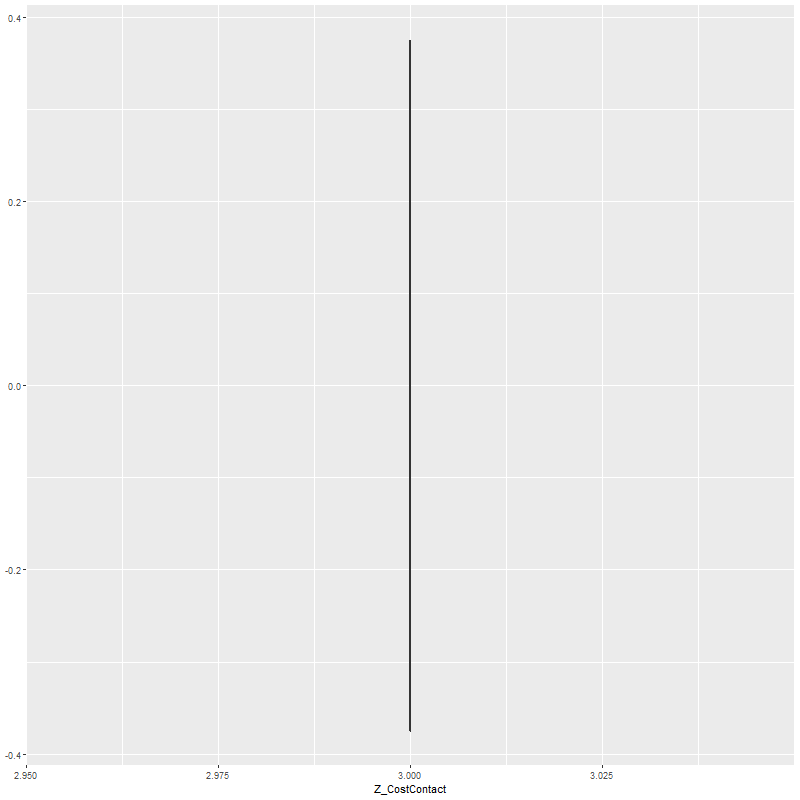
\includegraphics[width=\textwidth]{Img/DESCRIPTION018.png}
    \caption{BoxPlot Z\_CostContact}
    \label{fig:ZRevenue}
  \end{minipage}
  \hspace{5em}
  \begin{minipage}[b]{0.35\textwidth}
    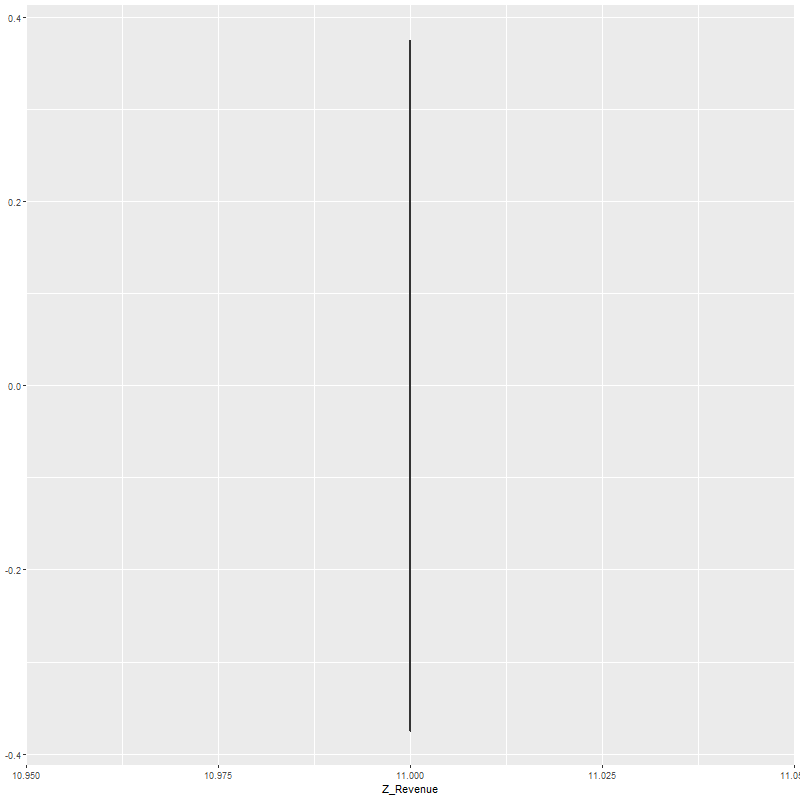
\includegraphics[width=\textwidth]{Img/DESCRIPTION019.png}
    \caption{BoxPlot Z\_Revenue}
      \label{fig:ZCostContact}
  \end{minipage}
\end{figure}
\end{frame}
%---------------------------------------------------------------------------%
\begin{frame}[fragile]
\frametitle{DataPreprocessing}
\begin{enumerate}
    \item Refactor del dataset
    \item Risoluzione dei valori mancanti nella variabile \textit{income}
    \item Splitting del dataset in \textit{trainingSet} e \textit{testSet}
    \item Feature Scaling
\end{enumerate}
\end{frame}
%---------------------------------------------------------------------------%
\begin{frame}[fragile]
\frametitle{Refactor del Dataset}
\begin{enumerate}
    \item Incorporamento dei dati ridondanti
    \item Conversione degli elementi in \textit{factor}
    \item Creazione di nuove variabili riassuntive
        \begin{itemize}
        \item Age
        \item Total\_Spent
        \item Total\_Campains
        \item Total\_Childs
    \end{itemize}
    \item Rimozione delle variabili superflue
    \begin{itemize}
        \item Z\_Revenue
        \item Z\_CostContact
        \item ID
        \item Dt\_customers
    \end{itemize}
\end{enumerate}
\end{frame}
%---------------------------------------------------------------------------%
\begin{frame}[fragile]
\frametitle{EDA}
\begin{figure}[!htb]
\minipage{0.32\textwidth}
  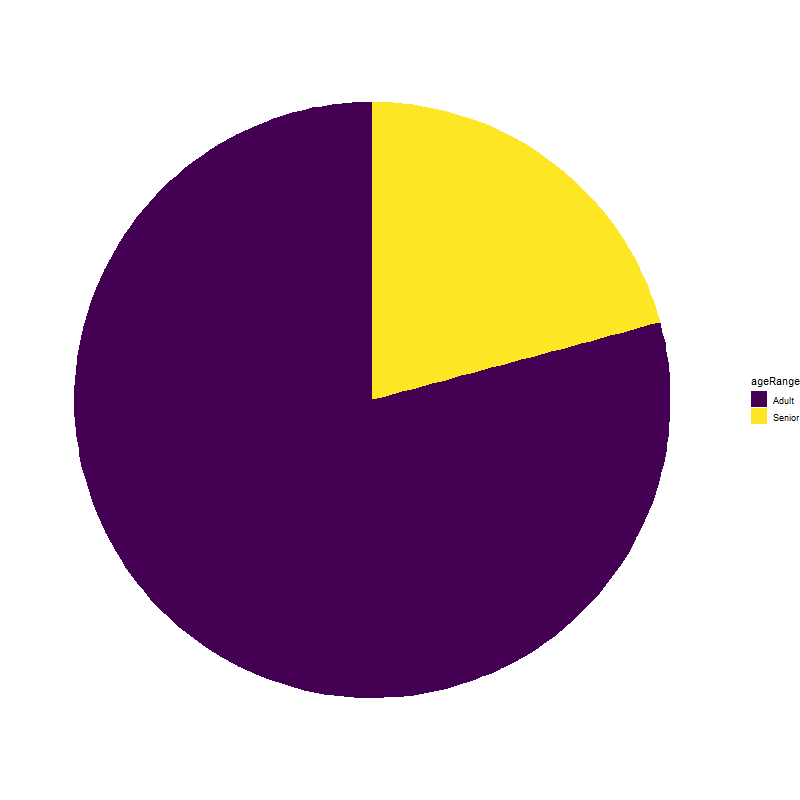
\includegraphics[width=\linewidth]{Img/eda/EDA001.png}
  \caption{Grafico a torta di \textit{Age}}\label{fig:PiePlotAge}
\endminipage\hfill
\minipage{0.32\textwidth}
  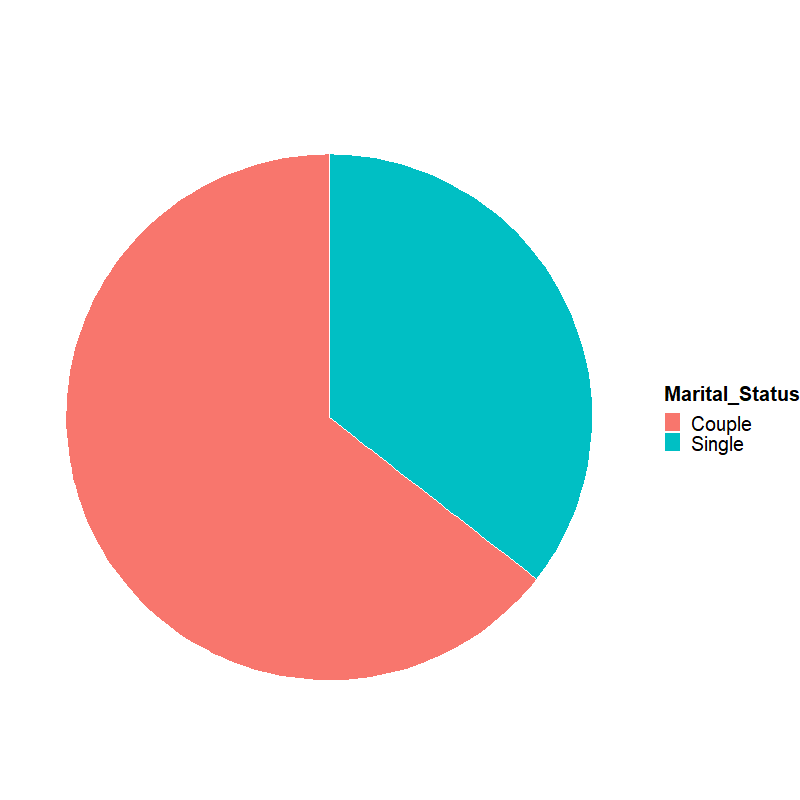
\includegraphics[width=\linewidth]{Img/eda/EDA002.png}
  \caption{Grafico a torta di \textit{Marital\_Status}}\label{fig:PiePlotMt}
\endminipage\hfill
\minipage{0.32\textwidth}%
  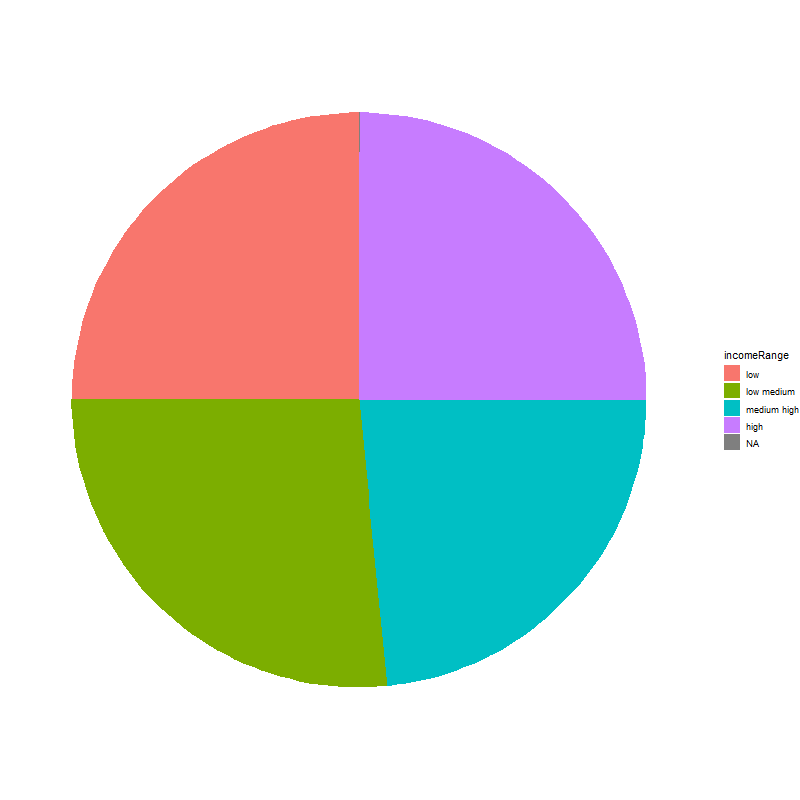
\includegraphics[width=\linewidth]{Img/eda/EDA003.png}
  \caption{Grafico a torta di \textit{Income}}\label{fig:PiePlotIncome}
\endminipage
\end{figure}
\end{frame}
%---------------------------------------------------------------------------%
\begin{frame}[fragile]
\frametitle{EDA: Age, Education  e Marital\_Status}
\begin{figure}[!htb]
\minipage{0.32\textwidth}
  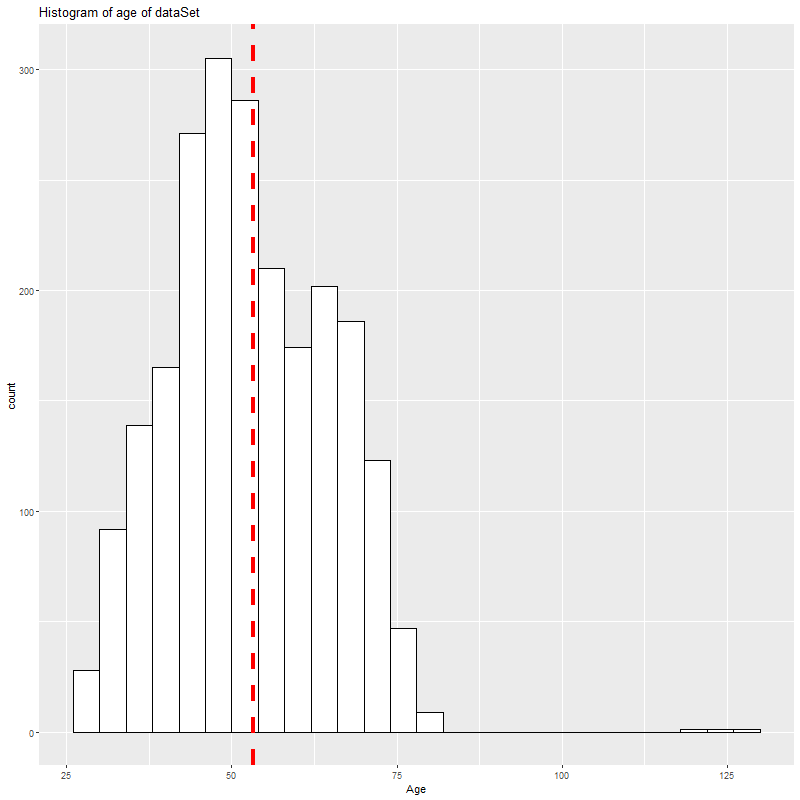
\includegraphics[width=\linewidth]{Img/eda/EDA005.png}
  \caption{Istogramma di \textit{Age}}\label{fig:HistPlotAge}
\endminipage\hfill
\minipage{0.32\textwidth}
  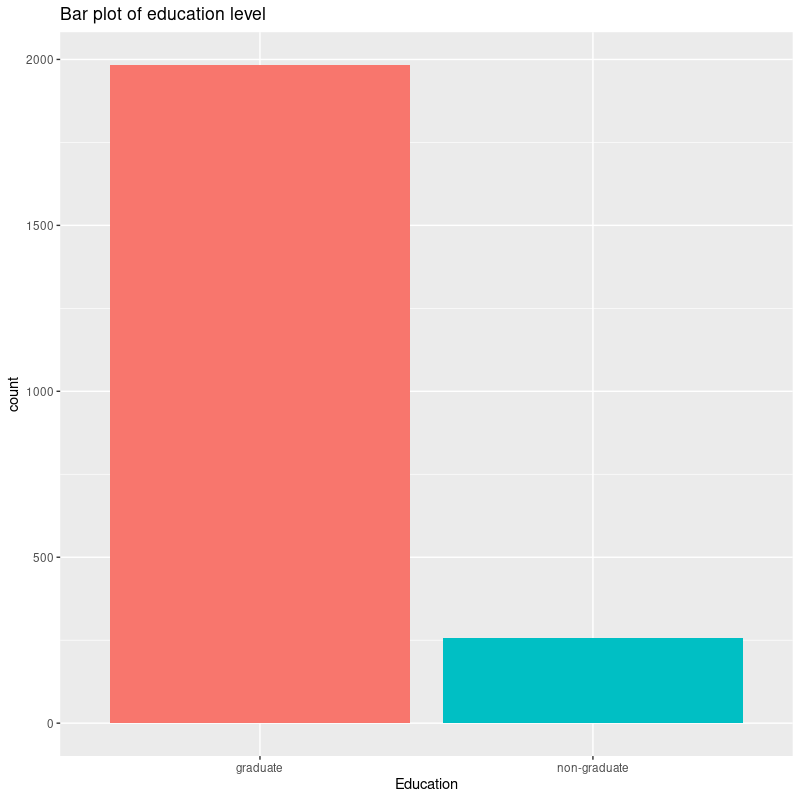
\includegraphics[width=\linewidth]{Img/eda/EDA007.png}
  \caption{Grafico a barre di \textit{Education}}\label{fig:BarPlotEducation}
\endminipage\hfill
\minipage{0.32\textwidth}%
  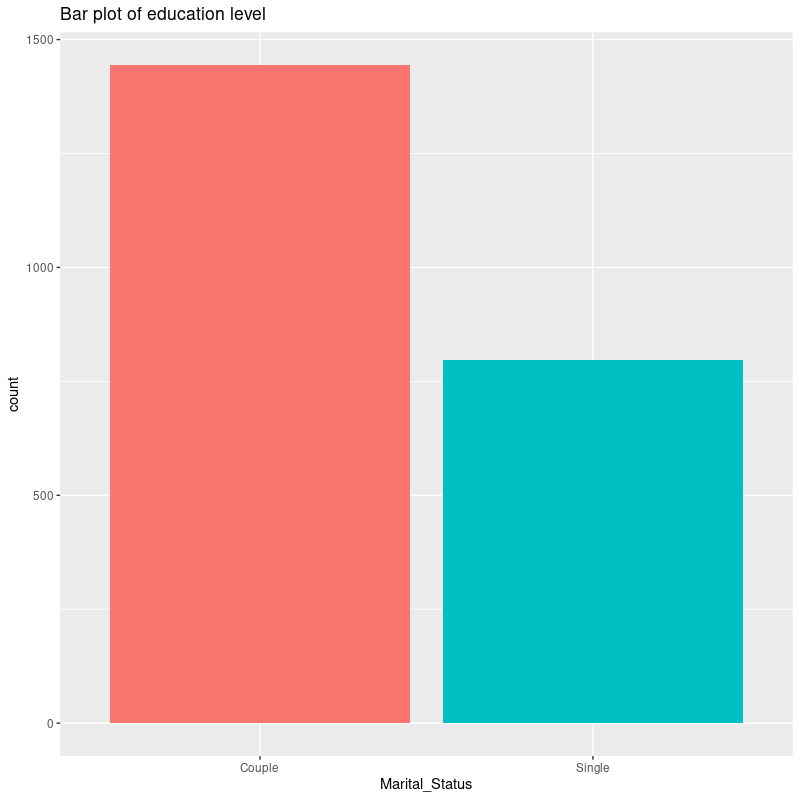
\includegraphics[width=\linewidth]{Img/eda/EDA051.png}
  \caption{Grafico a barre di \textit{Marital\_Status}}\label{fig:BarPlotMt}
\endminipage
\end{figure}
\end{frame}
%---------------------------------------------------------------------------%
\begin{frame}[fragile]
\frametitle{EDA: Istogrammi delle variabili Amount}

    \begin{figure}
    \centering
        \begin{minipage}{.3\textwidth}
            \begin{subfigure}{\textwidth}
            \centering
            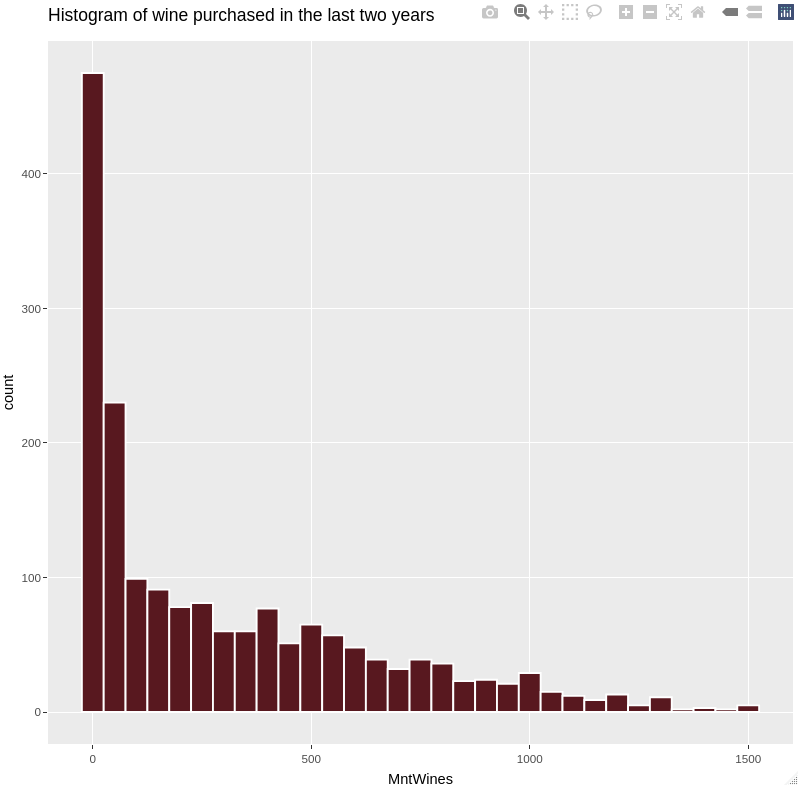
\includegraphics[width=0.7\textwidth]{Img/eda/EDA018.png}
            \end{subfigure}\\
            \begin{subfigure}{\textwidth}
            \centering
            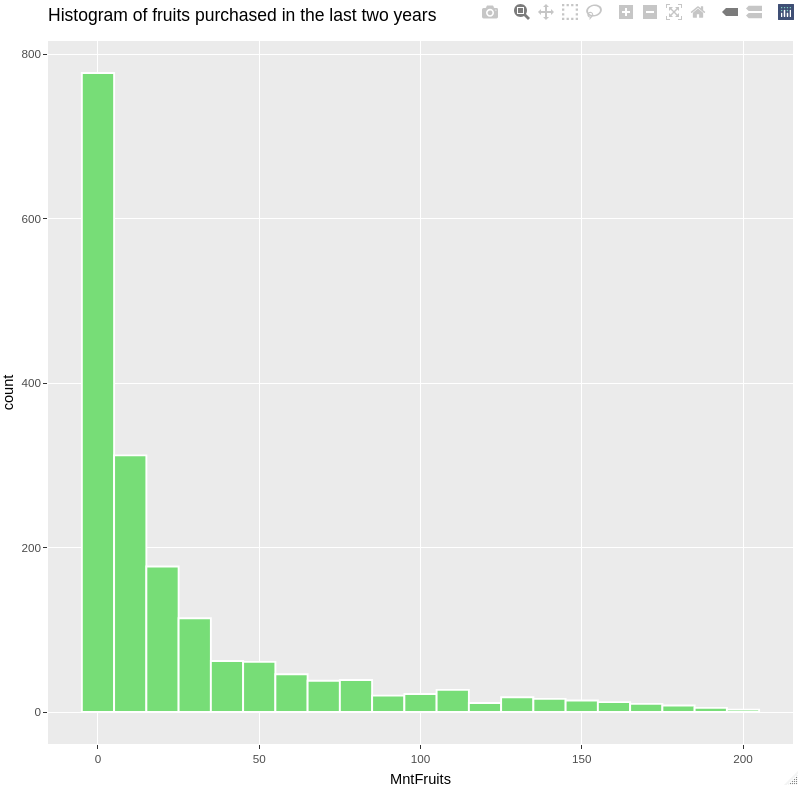
\includegraphics[width=0.7\textwidth]{Img/eda/EDA019.png}
            \end{subfigure}%    
        \end{minipage}
        \hfill
        \begin{minipage}{.3\textwidth}
            \begin{subfigure}{\textwidth}
            \centering
            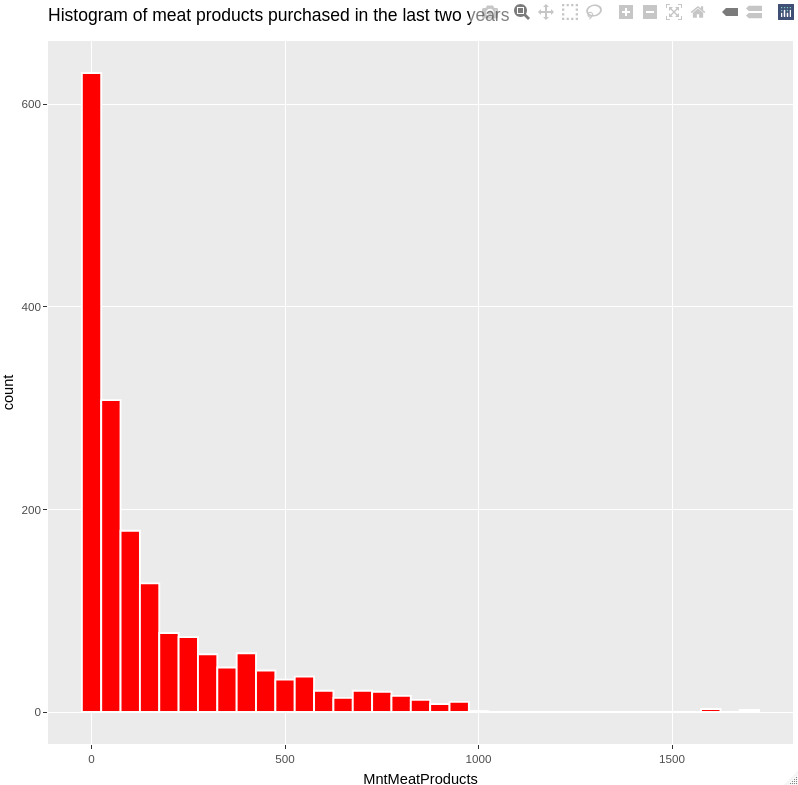
\includegraphics[width=0.7\textwidth]{Img/eda/EDA020.png}
            \end{subfigure}\\
            \begin{subfigure}{\textwidth}
            \centering
            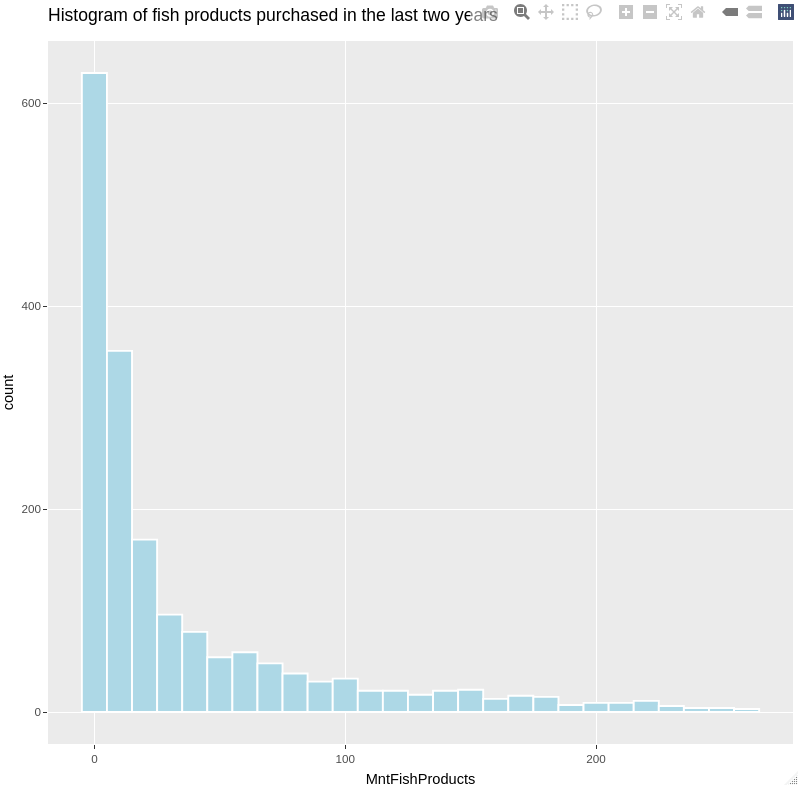
\includegraphics[width=0.7\textwidth]{Img/eda/EDA021.png}
            \end{subfigure}%   
        \end{minipage}
        \hfill
        \begin{minipage}{.3\textwidth}
            \begin{subfigure}{\textwidth}
            \centering
            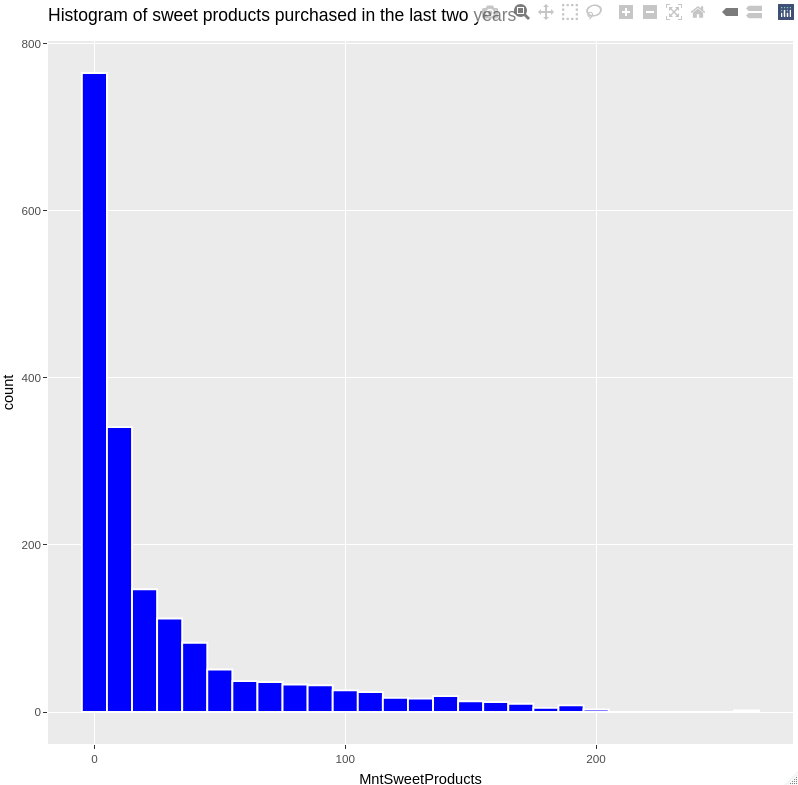
\includegraphics[width=0.7\textwidth]{Img/eda/EDA022.png}
            \end{subfigure}\\
            \begin{subfigure}{\textwidth}
            \centering
            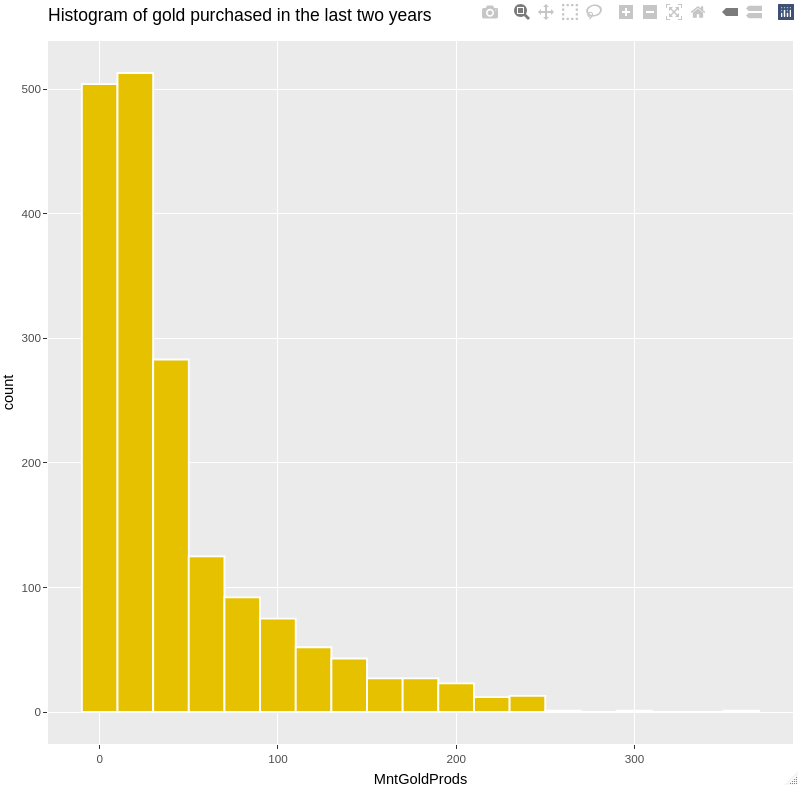
\includegraphics[width=0.7\textwidth]{Img/eda/EDA023.png}
            \end{subfigure}
        \end{minipage}%
    \end{figure}
\end{frame}
%---------------------------------------------------------------------------%
\begin{frame}[fragile]
\frametitle{EDA: Age, Education  e Marital\_Status}
\begin{figure}[!htb]
\minipage{0.32\textwidth}
  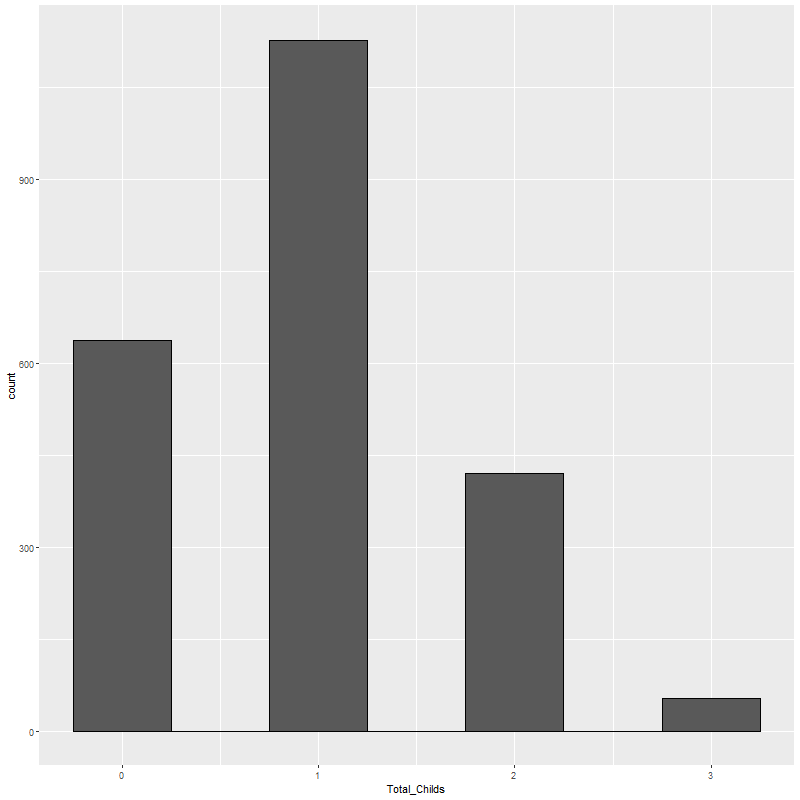
\includegraphics[width=\linewidth]{Img/eda/EDA009.png}
  \caption{Grafico a barre di \textit{Total\_Childs}}\label{fig:BarPlotTc}
\endminipage\hfill
\minipage{0.32\textwidth}
  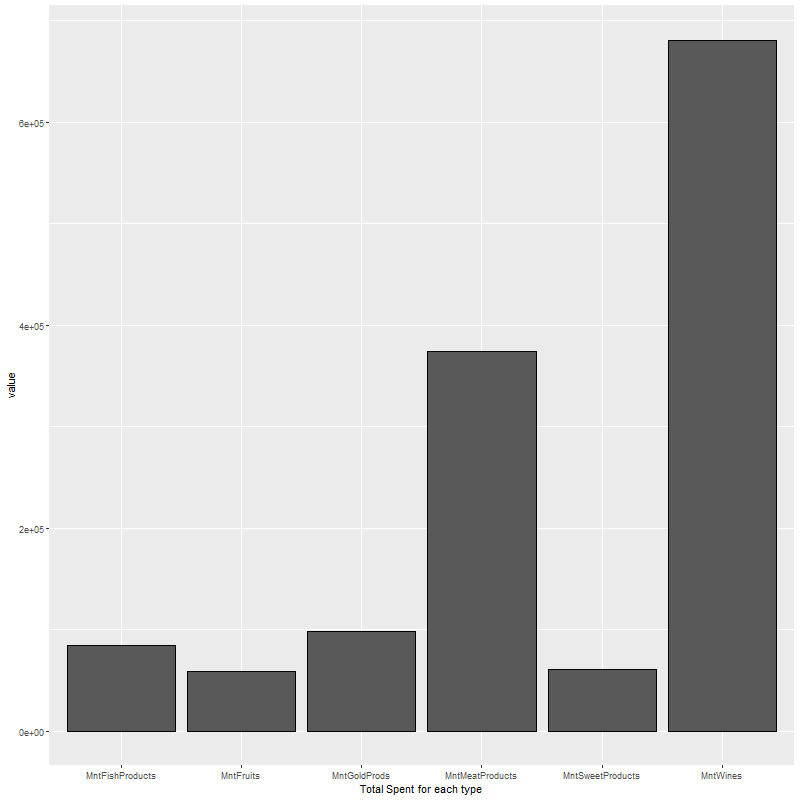
\includegraphics[width=\linewidth]{Img/eda/EDA017.png}
  \caption{Grafico a barre del totale speso per ogni tipo di prodotto}\label{fig:BarPlotTs}
\endminipage\hfill
\minipage{0.32\textwidth}%
  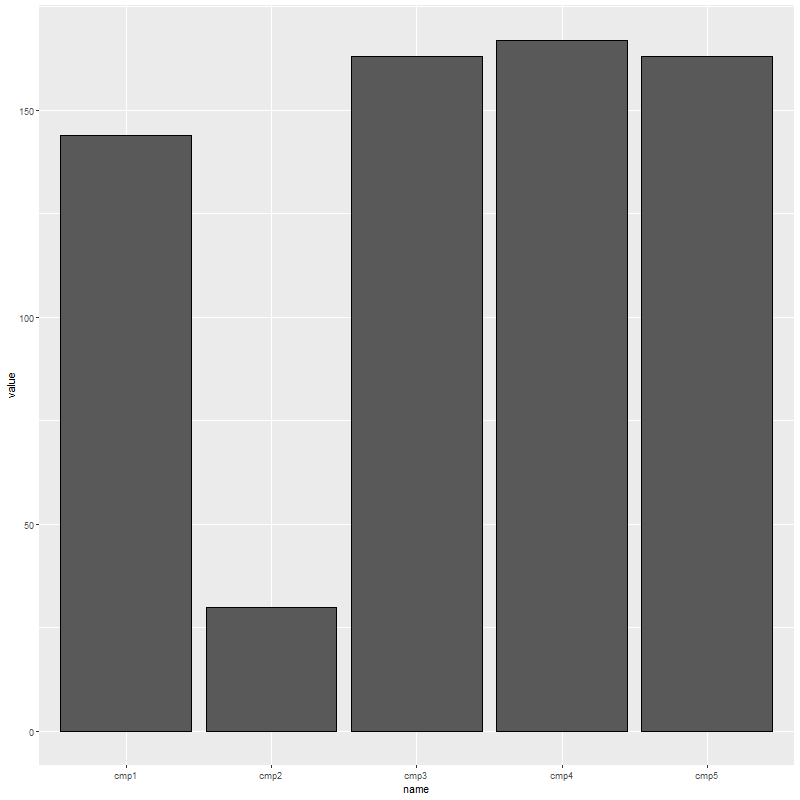
\includegraphics[width=\linewidth]{Img/eda/EDA045.png}
  \caption{Grafico a barre del totale di istanze che hanno accettato la campagna i-esima}\label{fig:BarPlotMt}
\endminipage
\end{figure}

\end{frame}
%---------------------------------------------------------------------------%
\begin{frame}[fragile]
\frametitle{PCA: Varianza spiegata da ogni dimensione}
\begin{minipage}{0.45\textwidth}
\begin{figure}[H]
    \centering
    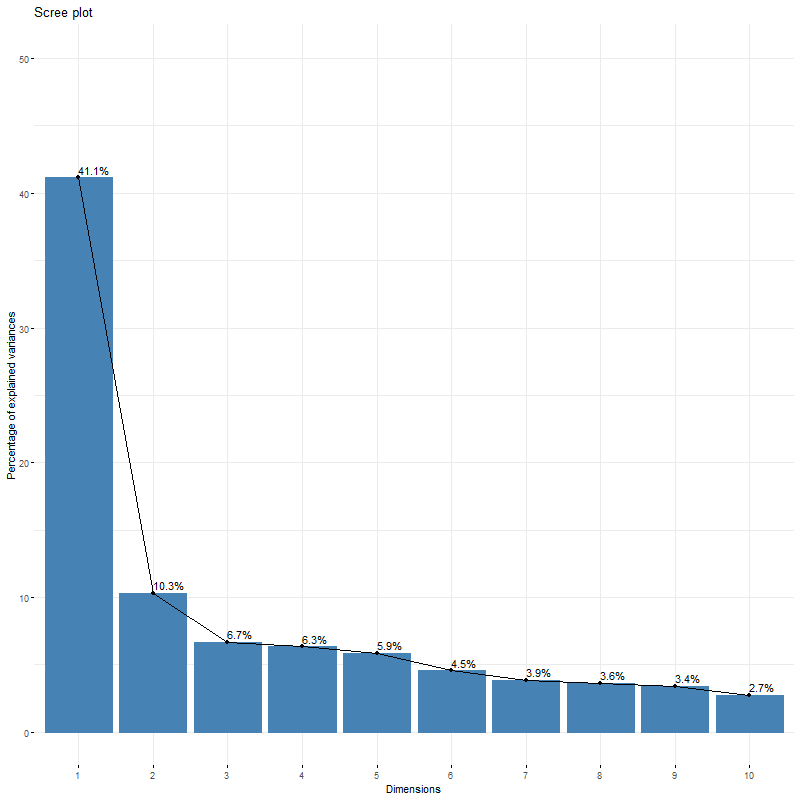
\includegraphics[width=0.8\textwidth]{Img/PCA001.png}
    \caption{Varianza spiegata da ogni Dimensione}
\end{figure}
\end{minipage}%
\hspace{2em}
\begin{minipage}{0.45\textwidth}
\begin{table}[H]
\centering
\begin{tabular}{rrrr}
  \hline
 & eig. & v.p. & c.v.p. \\ 
  \hline
Dim.1 & 7.00 & 41.15 & 41.15 \\ 
  Dim.2 & 1.75 & 10.31 & 51.46 \\ 
  Dim.3 & 1.14 & 6.69 & 58.15 \\ 
  Dim.4 & 1.08 & 6.34 & 64.49 \\ 
  Dim.5 & 1.00 & 5.86 & 70.34 \\ 
  ... & ... & ... & ... \\
   \hline
\end{tabular}
\caption{Output funzione \textit{get\_eigenvalue(pca)}}
\label{fig:get_eigenvalue(pca)}
\end{table}
\end{minipage}%
\end{frame}

%---------------------------------------------------------------------------%
\begin{frame}[fragile]
\frametitle{PCA: Varianza spiegata per la Dim1}
\begin{minipage}{0.45\textwidth}
\begin{figure}[H]
    \centering
    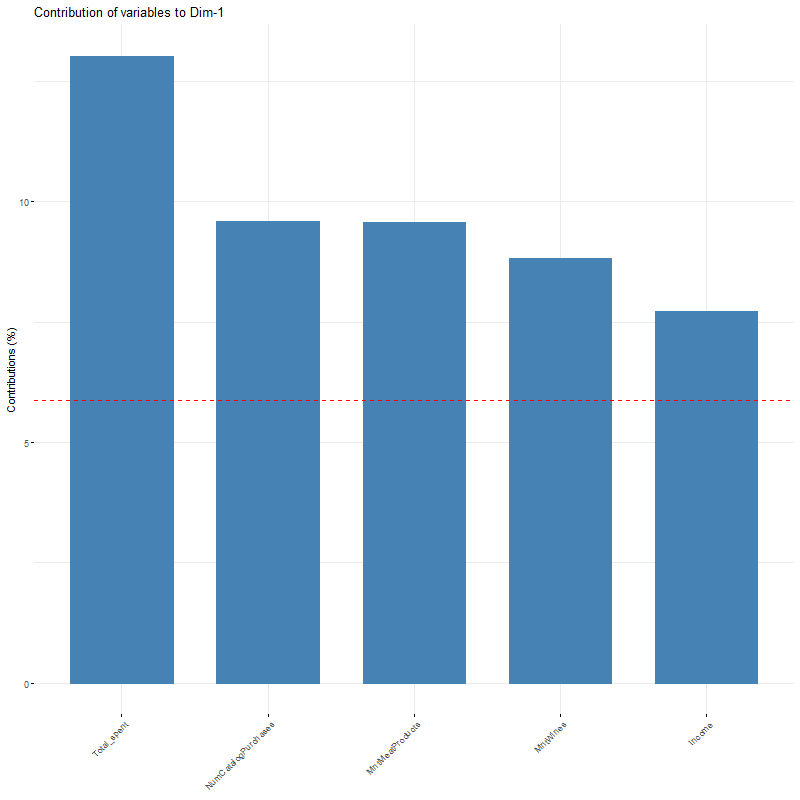
\includegraphics[width=0.7\textwidth]{Img/PCA002.png}
    \caption{Varianza spiegata dalle variabili per la prima dimensione}
    \label{fig:fviz_contrib(pca, choice = "var", axes = 1, top = 5)}
\end{figure}
\end{minipage}%
\hspace{3em}
\begin{minipage}{0.45\textwidth}
\begin{enumerate}
    \item Total\_Spent
    \item MntMeatProducts
    \item NumCatalogPurchases
    \item MntWines 
    \item Income
\end{enumerate}
\end{minipage}%
\end{frame}

%---------------------------------------------------------------------------%
% \begin{frame}[fragile]
% \frametitle{Creazione di nuove variabili riassuntive}
% \begin{table}[H]
% \centering
% \begin{tabular}{rrrr}
%   \hline
%  & Total\_spent & Total\_Campains & Total\_Childs \\ 
%   \hline
% 1 & 1617 &   0 &   0 \\ 
%   2 &  27 &   0 &   2 \\ 
%   3 & 776 &   0 &   0 \\ 
%   4 &  53 &   0 &   1 \\ 
%   5 & 422 &   0 &   1 \\ 
%   6 & 716 &   0 &   1 \\ 
%   \hline
% \end{tabular}
% \caption{Primi valori delle variabili Total\_spent \& Total\_Campains \& Total\_Childs}
% \label{fig:Totalspent&TotalCampains&TotalChilds}
% \end{table}

% \end{frame}


%---------------------------------------------------------------------------%
% \begin{frame}[fragile]
% \frametitle{Refactor: Eliminazione di dati ridondanti}
% \begin{minipage}{0.45\textwidth}
% \begin{table}[H]
% \centering
% \begin{tabular}{rl}
%   \hline
%  & unique(dataSet\$Marital\_Status) \\ 
%   \hline
% 1 & Single \\ 
%   2 & Together \\ 
%   3 & Married \\ 
%   4 & Divorced \\ 
%   5 & Widow \\ 
%   6 & Alone \\ 
%   7 & Absurd \\ 
%   8 & YOLO \\ 
%   \hline
% \end{tabular}
% \caption{Output $unique(dataSet\$Marital\_Status)$}
% \label{fig:unique(dataSetMaritalStatus)}
% \end{table}
% \end{minipage}%
% \hspace{2em}
% \begin{minipage}{0.45\textwidth}
% \begin{table}[H]
% \centering
% \begin{tabular}{rl}
%   \hline
%  & unique(dataSet\$Education) \\ 
%   \hline
% 1 & Graduation \\ 
%   2 & PhD \\ 
%   3 & Master \\ 
%   4 & Basic \\ 
%   5 & 2n Cycle \\ 
%   \hline
% \end{tabular}
% \caption{Output $unique(dataSet\$Education)$}
% \label{fig:unique(dataSetEducation)}
% \end{table}
% \end{minipage}%
% \end{frame}
% %---------------------------------------------------------------------------%
% \begin{frame}[fragile]
% \frametitle{Refactor: Eliminazione di dati ridondanti}
% \begin{minipage}{0.45\textwidth}
% \begin{table}[H]
% \centering
% \begin{tabular}{rl}
%   \hline
%  & unique(dataSet\$Education) \\ 
%   \hline
% 1 & graduate \\ 
%   2 & non-graduate \\ 
%   \hline
% \end{tabular}
% \caption{Output $unique(dataSet\$Education)$ dopo la procedura di \textit{collapsing} dei dati}
% \label{fig:unique(dataSetEducation)2}
% \end{table}
% \end{minipage}%
% \hspace{2em}
% \begin{minipage}{0.45\textwidth}
% \begin{table}[H]
% \centering
% \begin{tabular}{rl}
%   \hline
%  & unique(dataSet\$Marital\_Status) \\ 
%   \hline
% 1 & Single \\ 
%   2 & Couple \\ 
%   \hline
% \end{tabular}
% \caption{Output $unique(dataSet\$Marital\_Status)$ dopo la procedura di \textit{collapsing} dei dati}
% \label{fig:unique(dataSetMaritalStatus)2}
% \end{table}
% \end{minipage}%
% \end{frame}%
%---------------------------------------------------------------------------%
%->> Algoritmi
%---------------------------------------------------------------------------%
%---------------------------------------------------------------------------%
\lecture{Research Presentation}{lec_present_result}
%---------------------------------------------------------------------------%
\section{Algoritmi}
%---------------------------------------------------------------------------%
\begin{frame}[fragile]
\frametitle{Algoritmi scelti}
\begin{itemize}
    \item Supervisionato: \textbf{Decision Tree} 
    \item Non Supervisionato: \textbf{K-Means} 
\end{itemize}
\end{frame}

\begin{frame}[fragile]
\frametitle{Decision Tree}
\begin{minipage}{0.45\textwidth}
\begin{figure}
    \centering
    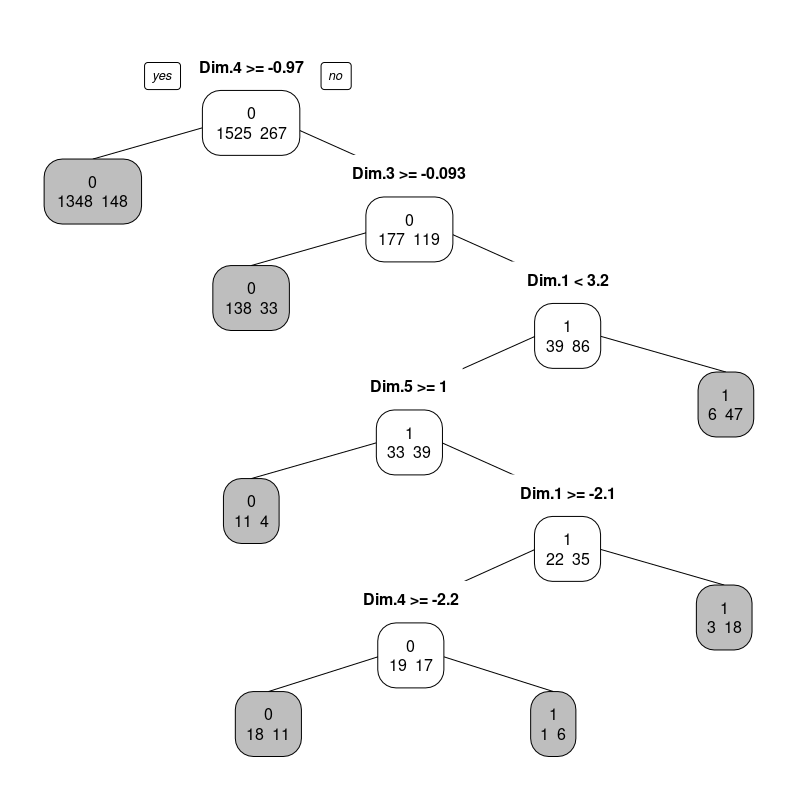
\includegraphics[width=0.8\textwidth]{Img/decision tree/D-TREE001.png}
    \caption{Decision Tree}
    \label{fig:DTREE1}
\end{figure}
\end{minipage}%
\hspace{2em}
\begin{minipage}{0.45\textwidth}

\begin{table}[h!]
\centering
\begin{tabular}{ll}
\multicolumn{2}{l}{\textbf{Positive Class:} 1} \\
\textbf{Accuracy:} 0.8348 & \textbf{Precision:} 0.1194\\
\textbf{Recall:} 0.3478 & \textbf{F-Measure:} 0.1777
\end{tabular}
\end{table}
\end{minipage}%
\end{frame}


\begin{frame}[fragile]
\frametitle{Decision Tree: Riduzione Overfitting}
\begin{minipage}{0.45\textwidth}
\begin{figure}
    \centering
    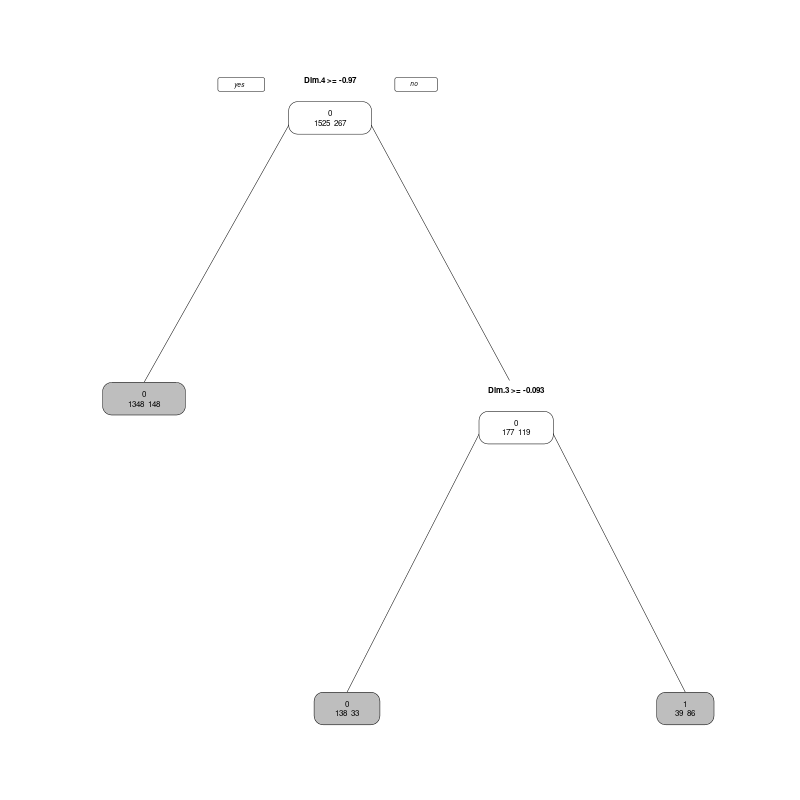
\includegraphics[width=0.8\textwidth]{Img/decision tree/D-TREE002.png}
    \caption{Decision Tree semplice}
    \label{fig:DTREE2}
\end{figure}
\end{minipage}%
\hspace{2em}
\begin{minipage}{0.45\textwidth}

\begin{table}[h!]
\centering
\begin{tabular}{ll}
\multicolumn{2}{l}{\textbf{Positive Class:} 1} \\
\textbf{Accuracy:} 0.8147 & \textbf{Precision:} 0.2777\\
\textbf{Recall:} 0.1492 & \textbf{F-Measure:} 0.1941
\end{tabular}
\end{table}

\end{minipage}%
\end{frame}

%
%---------------------------------------------------------------------------%
%->> Esperimenti
%---------------------------------------------------------------------------%
%---------------------------------------------------------------------------%
\lecture{Research Presentation}{lec_present_result}
%---------------------------------------------------------------------------%
\section{Esperimenti}
%---------------------------------------------------------------------------%

\begin{frame}[fragile]
\frametitle{Valutazione del modello: Decision Tree}
\begin{minipage}{0.45\textwidth}
\begin{figure}
    \centering
    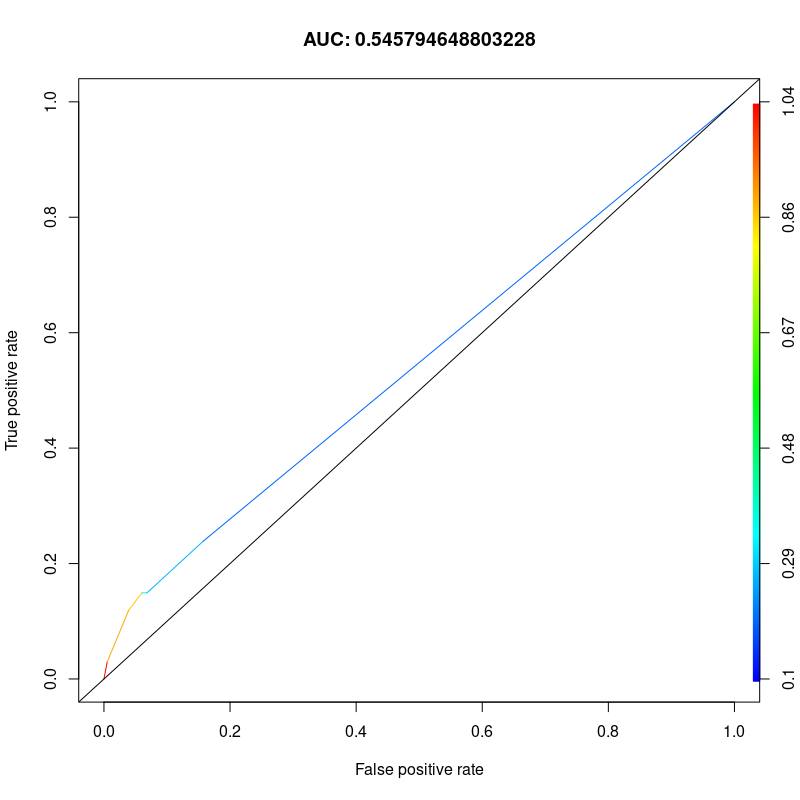
\includegraphics[width=0.8\textwidth]{Img/model evalutation/[D-TREE]ROC.png}
    \caption{Curva ROC}
    \label{fig:RocCurve}
\end{figure}
\end{minipage}%
\hspace{2em}
\begin{minipage}{0.45\textwidth}

\begin{table}[h!]
\centering
\begin{tabular}{|ll|lll|}
\hline
\multicolumn{2}{|l|}{\multirow{2}{*}{}} & \multicolumn{3}{l|}{Prediction}                        \\ \cline{3-5} 
\multicolumn{2}{|l|}{}                  & \multicolumn{1}{c|}{\_} & \multicolumn{1}{l|}{0}  & 1  \\ \hline
\multicolumn{2}{|l|}{\multirow{2}{*}{Reference}} & \multicolumn{1}{l|}{0} & \multicolumn{1}{l|}{1488} & 37 \\ \cline{3-5} 
\multicolumn{2}{|l|}{}                  & \multicolumn{1}{l|}{1} & \multicolumn{1}{l|}{200} & 67 \\ \hline
\end{tabular}
\end{table}

% \begin{table}[h!]
% \centering
% \begin{tabular}{ll}
% \textbf{Accuracy:} 0.8677 & \textbf{Precision:} 0.2509\\
% \textbf{Recall:} 0.6442 & \textbf{F-Measure:} 0.3611
% \end{tabular}
% \end{table}

\end{minipage}%
\end{frame}%
%---------------------------------------------------------------------------%
%->> Conclusion
%---------------------------------------------------------------------------%
%---------------------------------------------------------------------------%
\lecture{Research Presentation}{lec_present_conclude}
%---------------------------------------------------------------------------%
\section{Conclusioni}
%---------------------------------------------------------------------------%
\begin{frame}[fragile]
\frametitle{Conclusioni}
\begin{enumerate}
    \item K-Means
    \begin{itemize}
         \item Una buona suddivisione dei dati riportati può avvenire mediante l'utilizzo di due cluster.
    \item Il secondo cluster presenta clienti con un reddito generalmente al di sotto della media e sicuramente minore rispetto alla maggior parte dei compratori facenti parte della prima divisione.
    \item Riduzione delle spese totali da parte degli elementi all'interno del secondo gruppo.
    \end{itemize}
\end{enumerate}
\end{frame}

%%---------------------------------------------------------------------------%
%
%---------------------------------------------------------------------------%
%
%-
%-> Backmatter
%-
%---------------------------------------------------------------------------%
%->> Backmatter
%---------------------------------------------------------------------------%
%->> Question
%---------------------------------------------------------------------------%
\lecture{Research Presentation}{lec_present_question}
%---------------------------------------------------------------------------%
{%
\begin{frame}[plain]
    \begin{center}
        {\large\bfseries {Thank you for your attention!}}
    \end{center}
    \tikzart[t=p,x=0,y=-4,w=2]{logo_uw}
    \addtocounter{framenumber}{-1}% modify the counter to exclude a frame from total count
\end{frame}
}%
\end{document}
%---------------------------------------------------------------------------%
